\chapter{基本排版程序}
\begin{choices}
   1.下列关于质点的说法中,正确的是
   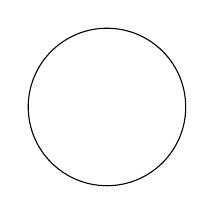
\begin{tikzpicture}
      \draw (0,0) circle [radius=1cm]; 
   \end{tikzpicture}
   A.质点是一个理想化的模型,实际上并不存在,所以引入这个概念没有多大意义
   B.体积很小的物体更容易看做质点
   C.凡轻小的物体,皆可看做质点凡轻小的物体,皆可看做质点凡轻小的物体,皆可看做质点凡轻小的物体,皆可看做质点
   D.当物体的形状和大小对所研究的问题属于无关或者次要因素时,即可把物体看成质点

   a.D

   e.建立理想模型是物理中的重要的研究方法,对于复杂问题的研究有重大意义,A错误;一个物体能否看做质点不应看其大小,关键是看其大小对于研究的问题的影响能否忽略,体积很小的物体有时可以看成质点,有时不能看成质点,B错误;一个物体能否看成质点不以轻重而论,C错误;物体能否看成质点取决于其大小和形状对所研究的问题是否属于无关或次要因素,若是就可以看成质点,D正确.
   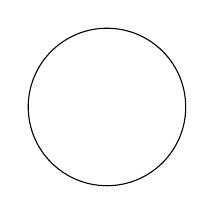
\begin{tikzpicture}
      \draw (0,0) circle [radius=1cm]; 
   \end{tikzpicture}
\end{choices}
这是附加的内容
这是附加的内容
这是附加的内容
是附加的内容
这是附加的内容
这是附加的内容
这是附加的内容
是附加的内容
是附加的内容
是附加的内容
这是附加的内容
这是附加的内容
这是附加的内容
这是附加的内容
这是附加的内容
这是附加的内容
这是附加的内容
这是附加的内容
这是附加的内容

 \begin{blanks}[exp]
  1.打点计时器是记录做直线运动物体的\blank{位移}和\blank{时间}的仪器,电火花计时器是其中的一种,其工作电压是\blank{220v},电火花计时器靠电火花和墨粉打点,当交流电的频率为$50Hz$ 时,它每隔\blank{0.02}秒打一次点。
 
 a.*
 
 e.此题考察打点计时器的应用与操作,打点计时器采用打点的方式在纸带上留下点迹,通过测量点迹间的距离可以确定位移。同时使用的电流一定是交流电,它每隔一段时间打一次点,通常频率为$50Hz$ 的交流电,每秒打点50次,所以每两次的间隔为$0.02s$.
 
 \end{blanks}

 \begin{blanks}
  1.用 $v-t$ 图像表示小车的运动情况时,以速度$v$ 为\blank{纵轴}、时间 $t$ 为\blank{横轴} 建立直角坐标系,用描点法画出小车的 $v-t$ 图象,图线的 \blank{斜率} 表示加速度的大小,如果 $v-t$ 图象是一条倾斜的直线,说明小车的速度是\blank{均匀变化}的。
 
 a.*
 
 e.此题考察 $v-t$ 图象的意义,通过 $v-t$ 图象识别加速度和判断物体运动特征。
 \end{blanks}

 \begin{proof}
    1. 设$x_1,x_2,\dots,x_n\geqslant 0$,且$x_1+x_2+\dots+x_n=\frac{1}{2}$ , 求证:
    \[
       (1-x_1)(1-x_2)\dots(1-x_n)\geqslant \frac{1}{2}
    \]

    p.由伯努利不等式得
    \[
       (1-x_1)(1-x_2)\dots(1-x_n)
       \geqslant
       1-(x_1+x_2+\dots+x_n)
       =1-\frac{1}{2}=\frac{1}{2}
    \]

   >pp.此题也是轮换不等式。由多元函数各偏微分为零可得,当$x_1=x_2=\dots=x_n$时,此多元函数取极值,即
    $x_i=\frac{1}{2n}$ ,于是
    \[
       f_m= (1-\frac{1}{2n})^n
    \]
    显然当$n$ 增加时,$fm$增加,同时由特殊值不可以写出此极值为极小值。同时极小值的极小值为$n=1$时,即 
    \[
       (1-x_1)(1-x_2)\dots(1-x_n)
       \geqslant
       (1-\frac{1}{2n})^n
       \geqslant
       \frac{1}{2}
    \]

 \end{proof}


2020年 07月 23日 星期四 07:27:49 CST
 证明环境设计思路,如果一下编辑多个证明题,则每个证明题后的前缀如果有*则此证明题加入证明结束符号。如果在环境结束前的一个题目中没有加*前缀,则结尾处自动加上结束符号。这样设计的原因是为了与amsthm.sty中所设置的数学证明环境相统一,在amsthm.sty中是一个环境处理一个问题,不涉及多个问题的连续处理,同时数学公式和图片不能混排。为了实现图片和数学文本的混排就得借助于cexam.sty,同时也支持多题目输入。这样就遇到了结束符号的输入问题,这需要谨慎设计。 

考虑到和amsthm.sty的兼容性,则仅在proof环境中加入证明结束标志,同时环境中如以>标志则此题结束,这是在amsthm.sty 的基础上进行的功能升级。其他的部分,由于按中文习题输入模式,则不再设置结束标志。
